\chapter{Ergebnisse}

\section{Präzision und Inferenzverhalten}

\subsection*{SSD}

Ursprünglich wurden 500 Epochen für das Training vorgesehen für jeden der Kreuzvalidierungsschritte. Da allerdings beim Training schon nach knapp über hundert Epochen sich der Gradient der Kostenfunktion nur träge veränderte, wurde im Sinne des \textit{Early Stoppings} nach 120 Epochen das Training vorzeitig beendet, um \textit{Overfitting} zu vermeiden. Das niedrigste Ergebnis der Kostenfunktion betrug 1.726. Es ergab eine \textit{mAP} von 83.1\%, leicht über den Referenzergebnissen von \textit{SSD} zu \textit{PascalVOC} (siehe Abbildung \ref{result}). Die Ergebnisse zu den einzelnen Klassen sind in folgender Tabelle dargestellt:

\begin{center}
	\begin{tabular}[h]{l|c}
		Klasse & mAP \\
		\hline
		Saskia Wasser Groß & 77.62\% \\
		Saskia Wasser Klein & 75.96\% \\
		Pepsi Cola Groß & 94.94\% \\
		Pepsi Cola Klein & 86.38\% \\
		ISO & 86.37\% \\
		ACE & 85.43\% \\
		Stenger Johannisbeerschorle & 69.47\% \\
		Stenger Apfelsaftschorle & 82.48 \% \\
		Vitamalz Malzbier & 76.24\%
	\end{tabular}
	\captionof{table}{Validierungsergebnisse SSD}
	\label{table:ssdresults}
\end{center}

Wird nun das trainierte Modell auf echte Daten angewendet, so fällt auf, dass manche Objekte doppelt detektiert werden. Um dieses Problem zu lösen, gibt es zwei Möglichkeiten. 

Als erstes kann bei der Detektion der minimale \textit{confidence score} angegeben werden, ab wann eine Detektion offiziell als solche wahrgenommen wird. Hier liegt die Herausforderung darin, einen optimalen Wert zu finden, sodass verdeckte Objekte noch als solche erkannt werden, aber doppelt erkannte Objekte nicht mehr auftreten. Der \textit{confidence score} wurde nach mehrmaligem Iterieren auf 0.75 festgelegt.

Die zweite Möglichkeit besteht darin, die maximale Überlappung zweier Bounding Boxen festzulegen. Somit werden doppelte Bounding Boxen, die sich flächenmäßig über einem gewissen Grenzwert überlappen, auf eine Bounding Box reduziert. Er stellte ich sich Parameter von 0.5 als geeignet heraus.

Außerdem wurden Inkonsistenzen im Detektionsverhalten festgestellt:

\begin{figure}[ht]
	\centering
	\subfigure[verdeckt]{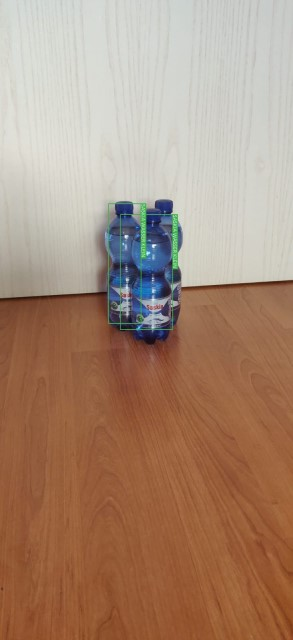
\includegraphics[width=0.30\textwidth]{Bilder/verdeckt.jpeg}}
	\hspace{2cm}
	\subfigure[winkel]{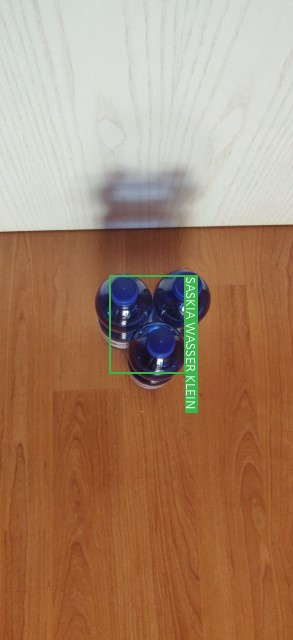
\includegraphics[width=0.30\textwidth]{Bilder/winkel.jpeg}}
	\caption{Detektionsverhalten bei extremen Blicklagen}
	\label{lagen}
\end{figure}

So sind von anderen Objekten verdeckte Objekte nur schwer zu erkennen, genauso wie Objekte aus extremen Blicklagen (siehe Abbildung \ref{lagen}). Diese Fälle wurden im Datensatz zwar zu 12.5\% abgedeckt, es lässt sich aber keine Aussage darüber treffen, ob eine Erweiterung des Datensatzes eine Abhilfe für dieses Problem hätte liefern können. 

\begin{figure}[ht]
	\subfigure[1 Meter]{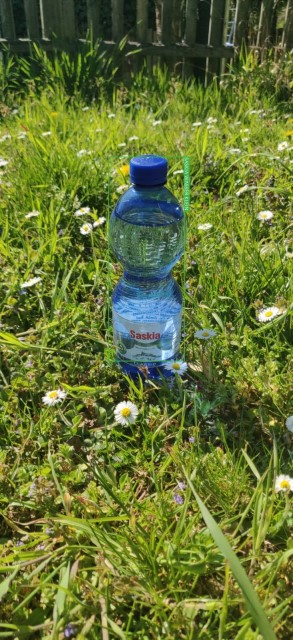
\includegraphics[width=0.30\textwidth]{Bilder/einmeter.jpeg}}\hfill
	\subfigure[2 Meter]{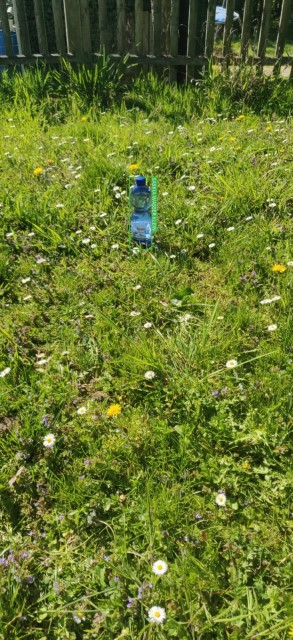
\includegraphics[width=0.30\textwidth]{Bilder/zweimeter.jpeg}}\hfill
	\subfigure[3 Meter]{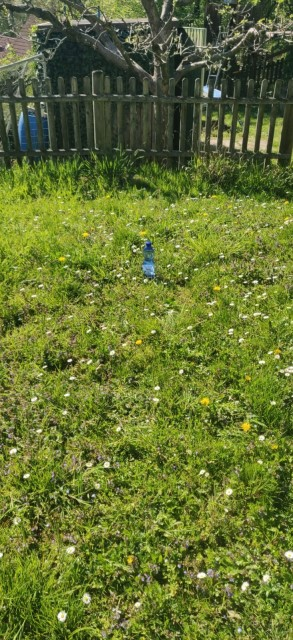
\includegraphics[width=0.30\textwidth]{Bilder/dreimeter.jpeg}}\hfill
	\caption{Detektionsverhalten bei unterschiedlichen Entfernungen}
	\label{entfernung}
\end{figure}

Auch die Entfernung zum zu detektierenden Objekt besitzt eine Auswirkung auf das Detektionsverhalten. In Abbildung \ref{entfernung} wird gezeigt, dass ab einer Entfernung von drei Metern keine Detektion mehr erfolgte. 

\begin{figure}[ht]
	\subfigure[überbeleuchtet]{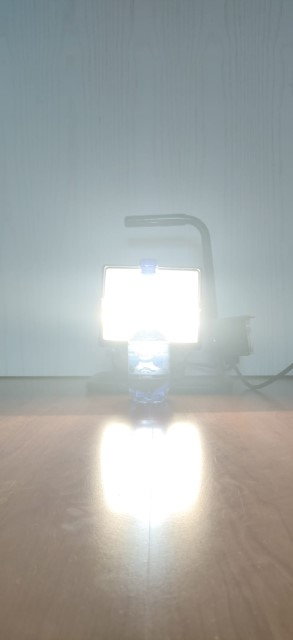
\includegraphics[width=0.30\textwidth]{Bilder/ueberbeleuchtet.jpeg}}\hfill
	\subfigure[normal]{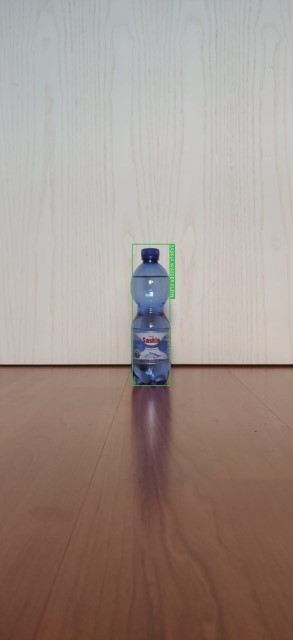
\includegraphics[width=0.30\textwidth]{Bilder/normalbeleuchtet.jpeg}}\hfill
	\subfigure[unterbeleuchtet]{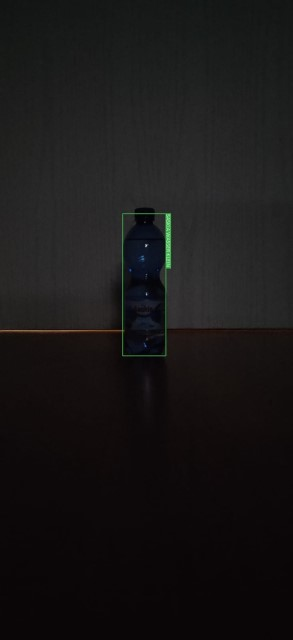
\includegraphics[width=0.30\textwidth]{Bilder/unterbeleuchtet.jpeg}}\hfill
	\caption{Detektionsverhalten bei unterschiedlichen Beleuchtungsverhältnissen}
	\label{sicht}
\end{figure}

Des Weiteren haben unterschiedliche Beleuchtungsgrade eine Auswirkung auf das Detektionsverhalten. In Abbildung \ref{sicht} wird unterschieden zwischen dem Detektionsverhalten bei überbeleuchteten, normalen und unterbeleuchteten Sichtverhältnissen. Überbeleuchtete Umgebungsverhältnisse erschweren die Objektdetektion in diesem Beispiel. 

Die Detektion reagierte allerdings invariant gegenüber unterschiedlichen Hintergründen oder Bildauflösungen.

\subsection*{YOLO}

Das Training von \textit{YOLO} ergab eine \textit{mAP} von 80.36\%. Abbildung \ref{yolo_result} zeigt die Verbesserung des Modells während dem Trainingsprozess. Es fällt auf, dass nach etwa 3600 Batches (umgerechnet circa 230 Epochen) bereits eine \textit{mAP} von 79\% erreicht wurde.

\begin{figure}[ht]
	\begin{center}
		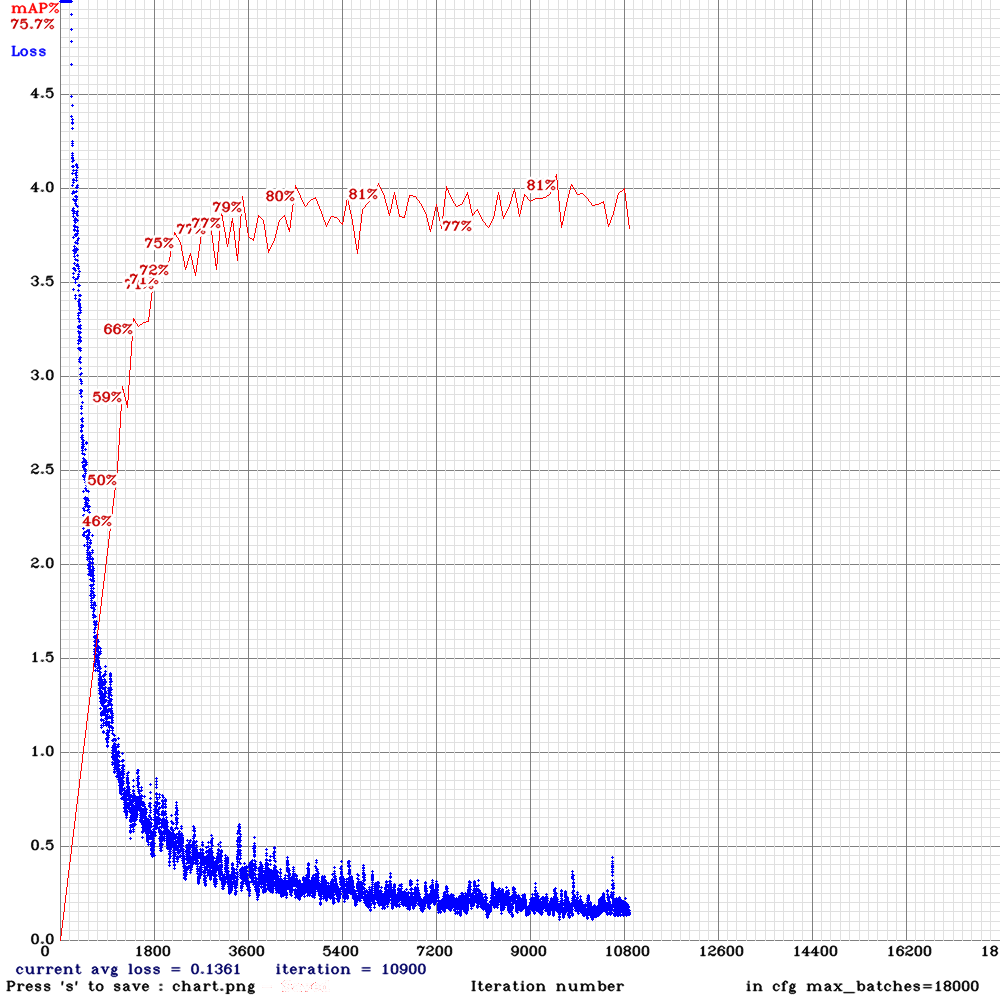
\includegraphics[width=13cm]{Bilder/yolo_result.png} 
		\caption{Aufzeichnung des Trainingsprozess von \textit{YOLO}}
		\label{yolo_result}
	\end{center}
\end{figure}

\begin{center}
	\begin{tabular}[h]{l|c}
		Klasse & mAP \\
		\hline
		Saskia Wasser Groß & 76.69\% \\
		Saskia Wasser Klein & 80.63\% \\
		Pepsi Cola Groß & 73.14\% \\
		Pepsi Cola Klein & 75.24\% \\
		ISO & 90.28\% \\
		ACE & 86.69\% \\
		Stenger Johannisbeerschorle & 72.50\% \\
		Stenger Apfelsaftschorle & 78.05 \% \\
		Vitamalz Malzbier & 81.94\%
	\end{tabular}
	\captionof{table}{Validierungsergebnisse YOLO}
	\label{table:yoloresults}
\end{center}

TODO:
 - verlgeiche wie bei SSD
 
 
\section{Reaktionsvermögen}

Bei der Inferenz fällt allerdings entgegen der Erwartungen auf, dass die Inferenz überdurchschnittlich langsam verläuft. Das Problem lässt sich auf die synchrone Arbeitsweise der bisherigen Detektionsalgorithmen zurück führen, bei dem erst ein neuer Frame des Videostreams angefragt wird, sobald das aktuelle Bild durch die Vorverarbeitung gelaufen ist und durch das Modell inferiert wurde. 

Um dem entgegen zu wirken, wurde ein Bufferkonzept in einem parallelem Thread realisiert, der einzelne Frames zeitgleich zur Inferenz anfragt und zwischenspeichert. Ist der Buffer voll, so werden nach dem \textit{First In First Out} Verfahren die älteren Frames verworfen. Dadurch konnte die FPS Anzahl von \textit{SSD} von maximal 18 auf die vollen 30 gesteigert werden. 

Ein weiteres Problem beschreibt die initiale Latenz zwischen der Inferenz und der Bildaufnahme. Die Inferenz kann erst gestartet werden, sobald die Gewichtungen des Modells initialisiert wurden. Dies lässt sich umgehen, indem entweder der Thread zur Bildaufnahme verzögern gestartet wird oder dessen Buffer kleiner gewählt wird.

\section{Trainingsverhalten}


